%%%%%%%%%%%%%%%%%%%%%%%%%%%%%%%%%%%%%%%%%%%%%%%%%%%%%%%%%%%%%%%%%%%%%%
% How to use writeLaTeX:
%
% You edit the source code here on the left, and the preview on the
% right shows you the result within a few seconds.
%
% Bookmark this page and share the URL with your co-authors. They can
% edit at the same time!
%
% You can upload figures, bibliographies, custom classes and
% styles using the files menu.
%
% If you're new to LaTeX, the wikibook is a great place to start:
% http://en.wikibooks.org/wiki/LaTeX
%
%%%%%%%%%%%%%%%%%%%%%%%%%%%%%%%%%%%%%%%%%%%%%%%%%%%%%%%%%%%%%%%%%%%%%%
\documentclass{tufte-handout}

%\geometry{showframe}% for debugging purposes -- displays the margins

\usepackage{amsmath}

% Set up the images/graphics package
\usepackage{graphicx}
\setkeys{Gin}{width=\linewidth,totalheight=\textheight,keepaspectratio}
\graphicspath{{graphics/}}

\title{Hands-On Session: Data Encryption}
\author{DIME Analytics \\ dimeanalytics@worldbank.org}
\date{11 June 2019}  % if the \date{} command is left out, the current date will be used

% The following package makes prettier tables.  We're all about the bling!
\usepackage{booktabs}

% The units package provides nice, non-stacked fractions and better spacing
% for units.
\usepackage{units}

% The fancyvrb package lets us customize the formatting of verbatim
% environments.  We use a slightly smaller font.
\usepackage{upquote}
\usepackage{fancyvrb}
\fvset{fontsize=\normalsize}
\renewcommand{\FancyVerbFormatLine}{\color{violet}}
\DefineShortVerb{\|}

% Small sections of multiple columns
\usepackage{multicol}

% Provides paragraphs of dummy text
\usepackage{lipsum}

 \usepackage{float}

% These commands are used to pretty-print LaTeX commands
\newcommand{\doccmd}[1]{\texttt{\textbackslash#1}}% command name -- adds backslash automatically
\newcommand{\docopt}[1]{\ensuremath{\langle}\textrm{\textit{#1}}\ensuremath{\rangle}}% optional command argument
\newcommand{\docarg}[1]{\textrm{\textit{#1}}}% (required) command argument
\newenvironment{docspec}{\begin{quote}\noindent}{\end{quote}}% command specification environment
\newcommand{\docenv}[1]{\textsf{#1}}% environment name
\newcommand{\docpkg}[1]{\texttt{#1}}% package name
\newcommand{\doccls}[1]{\texttt{#1}}% document class name
\newcommand{\docclsopt}[1]{\texttt{#1}}% document class option name

\begin{document}

\maketitle% this prints the handout title, author, and date

\begin{marginfigure}%
  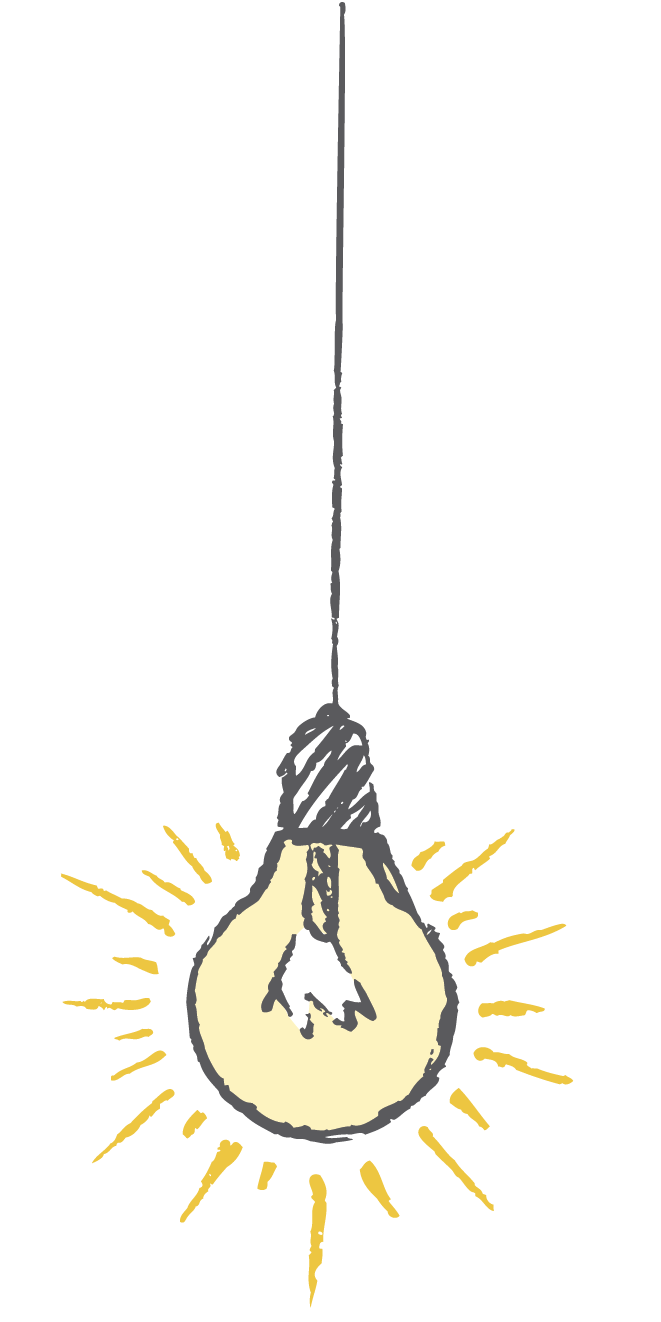
\includegraphics[width=\linewidth]{img/light.png}
\end{marginfigure}

\begin{abstract}
In this exercise we will encrypt a dataset and attempt to access the data in an encrypted folder

\bigskip\noindent \textbf{Exercise Objectives}: On completing this exercise you will be able to
\begin{enumerate}
  \item Download and install VeraCrypt
  \item Set up a secure folder using VeraCrypt
  \item Encrypting files in the secure folder
  \item Access the encrypted files in the secure folder
\end{enumerate}
\end{abstract}

%\printclassoptions
\section{Part 1: Download and install VeraCrypt}

VeraCrypt is the software that we recommend when encrypting data on your computer, regardless if it is an a non-shared folder, or a shared folder like DropBox. VeraCrypt is a free open-source software so you can use it without having to pay for it.

The first time we use VeraCrypt we need to download and install the software. If you are using a World Bank desktop, then you must make an \textit{eServices} request and have an IT person installing the software for you.

If you are not using World Bank computer, then you can download the software here: \url{https://www.veracrypt.fr/en/Downloads.html}. For Mac computers there is the installer version, chose that one. For Windows users there are 4 version, chose the \textit{installer}-version. After you have downloaded the installer file, open it and follow the instructions. Most people do not need to change any of the default values.

Anyone in your team that want to access the files you encrypt with VeraCrypt will also have to download the software to be able to access the files.

\section{Part 2: Set up VeraCrypt}

Before you can encrypt any files on your computer you must use VeraCrypt to create a special folder. In VeraCrypt this is called a \textit{Volume} but think of this as a very secure folder that you access in a different way.

\begin{enumerate}

	\item If you have VeraCrypt open, start by closing it, and re-open it. All our instructions will start from the opening page.
	\item On the opening page click \textit{Create Volume} (marked in read in the image below). Remember that \textit{Volume} in VeraCrypt means secure folder.
	\begin{figure}%
		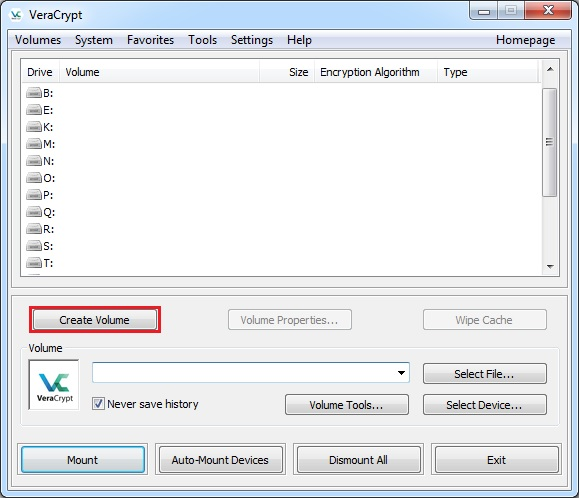
\includegraphics[width=.9\linewidth]{img/vc_install_1.png}
	\end{figure}
	\FloatBarrier
		
	\item In \textit{The VeraCrypt Volume Creation Wizard} you have three options. VeraCrypt has many very advanced options, but for the type of work we do we will only use the simplest option which is creating \textit{encrypted file container} type of volumes which is the default option.
	
	\begin{figure}
		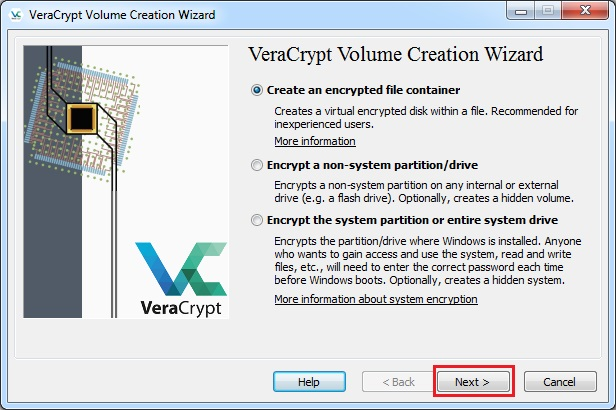
\includegraphics[width=.9\linewidth]{img/vc_install_2.png}
	\end{figure}
	\FloatBarrier
	
	\newpage
	
	\item In the next step we will again chose the simplest options and create a \textit{Standard VeraCrypt volume} and then click \textit{Next}.
	\begin{figure}
		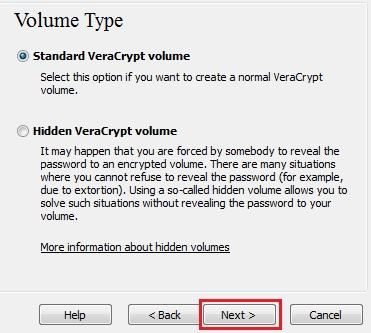
\includegraphics[width=.75\linewidth]{img/vc_install_3.png}
	\end{figure}
	\FloatBarrier
	
	\item Next you have to specify where you want to create the secure folder \textit{volume}. The volume behaves as a folder where you can store files, but technically it is a file (you do not need to understand how it works). So chose a location and give the volume file a name. Click select file. \sidenote{Note that a VeraCrypt container is just like any normal file. It can be, for example, moved or deleted as any normal file.}
	\begin{figure}%
		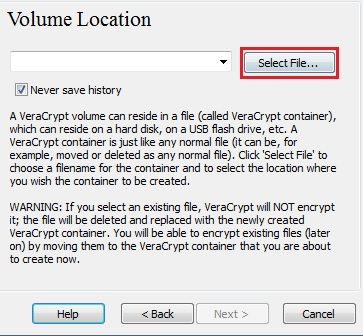
\includegraphics[width=.75\linewidth]{img/vc_install_4.png}
	\end{figure} 
	\FloatBarrier
	
	\newpage
	
	\item Select the desired path in the file selector,. If you intend to share this folder, for example through DropBox, then this should be inside your DropBox folder. If you are using DIME Analytics' folder set-up then you should create this inside the encrypted folder.\sidenote{\url{https://dimewiki.worldbank.org/wiki/DataWork_Folder\#Survey_Encrypted_Data}}. Then type the name of the secure folder in the \textit{file name} box (remember the secure folder volume is actually a file), and then click \textit{Save}.
	
	\begin{figure}%
		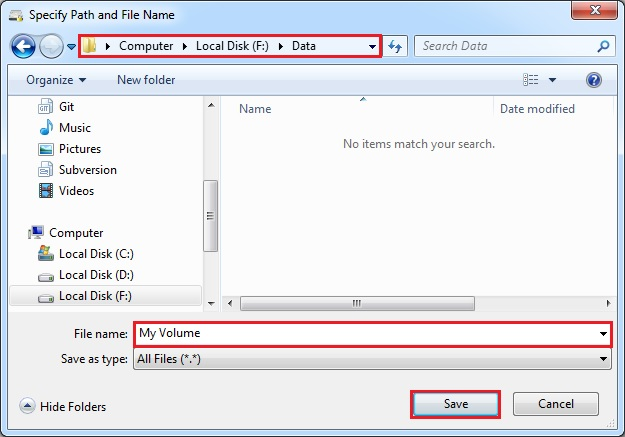
\includegraphics[width=.8\linewidth]{img/vc_install_5.png}
	\end{figure}
	\FloatBarrier
	
	
	\item Back in the \textit{Volume Creation Wizard} window, click \textit{Next}.
	\begin{figure}%
		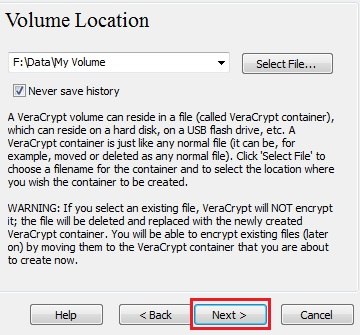
\includegraphics[width=.8\linewidth]{img/vc_install_6.png}
	\end{figure}
	\FloatBarrier
	
	\newpage
	
	\item One of the restrictions of VeraCrypt is that you already at this stage need to decide what the maximum size of the secure folder will be. Do not exaggerate to much, as the secure folder will always take up this much disk space, even when it is empty.\sidenote{If you end up choosing too small volume size you can in the future create a new larger volume and move the files there.} In this example, chose 250 megabyte and then click \textit{Next}.
	\begin{figure}%
		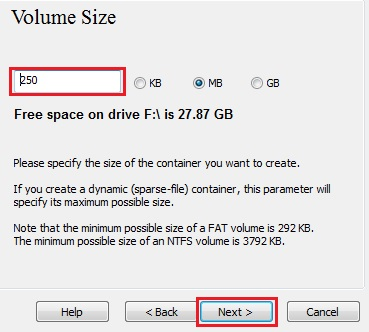
\includegraphics[width=.7\linewidth]{img/vc_install_7.png}
	\end{figure}
	\FloatBarrier
	
	
	\item In the next step you need to create a secure password.\sidenote{We recommend using a password manager like LastPass \url{https://www.lastpass.com/}. If you are working in a World Bank project you can get access to LastPass Premium version for free, but the basic version that is free for everyone will suit all your needs for this purpose.} Read VeraCrypt's instructions for what is a good password. After you have chosen your password, type it in the first input field and then re-type it in the second input field, and then click \textit{Next}.
	\begin{figure}%
		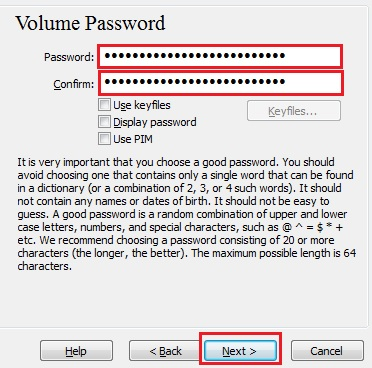
\includegraphics[width=.7\linewidth]{img/vc_install_8.png}
	\end{figure}
	\FloatBarrier
	
	
	\item To make the encryption completely unpredictable, VeraCrypt use your mouse movement to get a random input. Move your mouse inside the VeraCrypt window until the randomness indicator becomes green. The longer you move the mouse, the better. Then click \textit{Format}.
	\begin{figure}%
		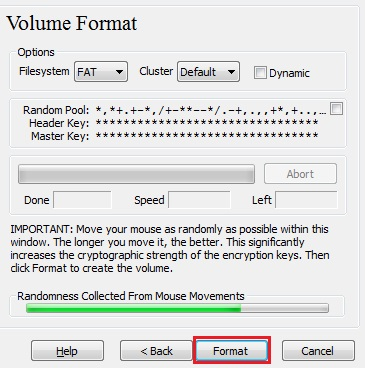
\includegraphics[width=.7\linewidth]{img/vc_install_9.png}
	\end{figure}
	\FloatBarrier
\end{enumerate}

	\noindent You have now created the secure folder. Go to the location where you created the folder to confirm it exists. It does not look like a folder, as it is technically a file. Double click on the folder to try and open it directly. Confirm that it doesn't open and you cannot do anything with it. Also see that the file is about 250MB big (or whatever value you chose) despite it is still empty.

%\printclassoptions
\section{Part 2: Adding files to your secure folder}
\begin{enumerate}
	\item Open VeraCrypt.
	\item Mount the encrypted volume created onto drive M. \\
	\textit{Note that, you can use any drive of your choice.}
	\begin{itemize}
		\item  Select a drive letter from the list (marked with a red rectangle). This will be the drive letter to which the VeraCrypt container will be mounted.
	\end{itemize}
	\begin{figure}%
		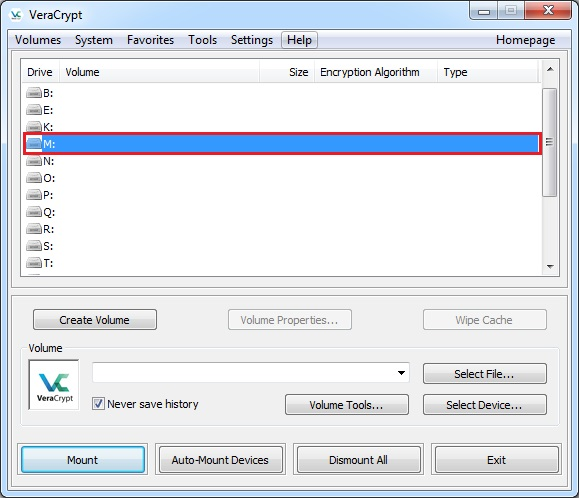
\includegraphics[width=\linewidth]{img/vc_mount_1.png}
	\end{figure}
	\FloatBarrier
	\begin{itemize}
		\item  Click Select File.
	\end{itemize}
	\begin{figure}%
		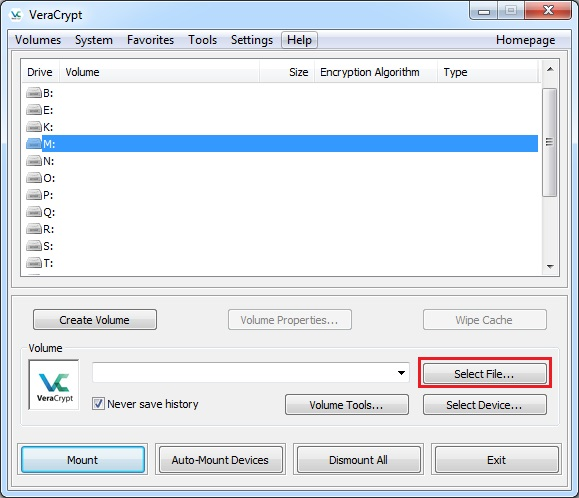
\includegraphics[width=\linewidth]{img/vc_mount_2.png}
	\end{figure}
	\FloatBarrier	
	\begin{itemize}
		\item In the file selector, browse to the container file (which we created earlier)and select it. Click Open (in the file selector window).
	\end{itemize}
	\begin{figure}%
		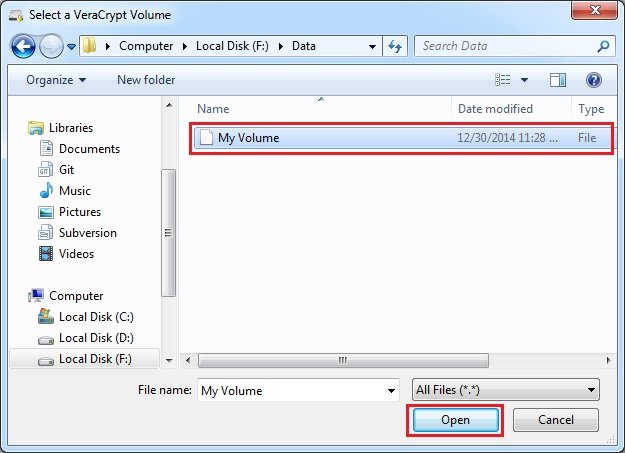
\includegraphics[width=\linewidth]{img/vc_mount_3.png}
	\end{figure}
	\FloatBarrier
	\begin{itemize}
		\item In the main VeraCrypt window, click Mount. Password prompt dialog window should appear.
	\end{itemize}
	\begin{figure}%
		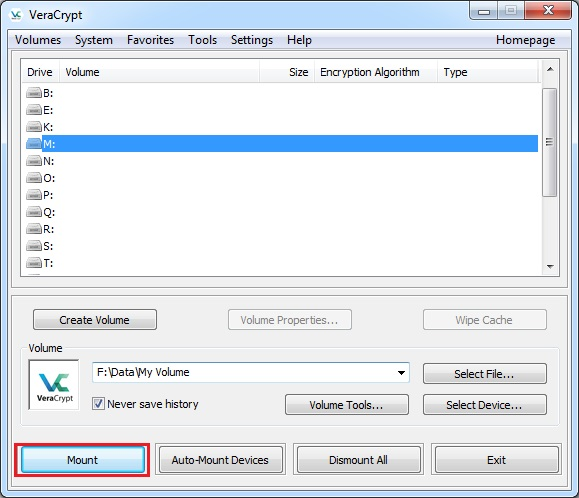
\includegraphics[width=\linewidth]{img/vc_mount_4.png}
	\end{figure}
	\FloatBarrier
	\begin{itemize}
		\item Type the password (which you specified in Step 10) in the password input field (marked with a red rectangle). Click OK.
	\end{itemize}
	\begin{figure}%
		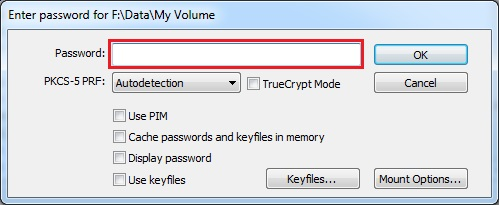
\includegraphics[width=\linewidth]{img/vc_mount_5.png}
	\end{figure}
	\FloatBarrier
	\begin{itemize}
		\item If the password is correct, we will have successfully mounted on the container as a virtual disk M:. Double click on the disk M: to open the container. 
	\end{itemize}
	\begin{figure}%
		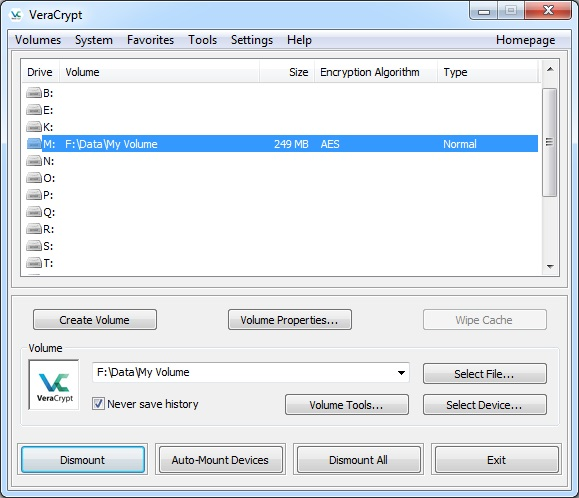
\includegraphics[width=\linewidth]{img/vc_mount_6.png}
	\end{figure}
	\FloatBarrier
	\item This will now open an empty folder titled 'Encrypted Data'. Save a copy of the data sets titled endline\_data\_raw\_2018.dta and endline\_data\_raw\_nodup\_2018.dta\sidenote{Update to final dataset once ready} in the folder. \\
	\textit{This is very similar to using a new USB/flash drive and adding files to it.}
	\item Open VeraCrypt and dismount the drive.
	\item Share the password securely with team members.\sidenote{Add something about securely sharing passwords}
	
	
\end{enumerate}


%\printclassoptions
\section{Part 3: Access encrypted files}
\begin{enumerate}
	\item Open VeraCrypt.
	\item Mount the encrypted volume created onto drive K. \\
	\textit{Note that, you can use any drive of your choice.}
	\item This will now open a folder titled 'Encrypted Data' which contains the data sets titled endline\_data\_raw\_2018.dta and endline\_data\_raw\_nodup\_2018.dta\sidenote{Update to final dataset once ready}.
	\item Open VeraCrypt and dismount the drive   
\end{enumerate}

NOTE: When calling a file in the encrypted folder on Stata the file path used will be that of the mounted drive and not that of where the encrypted file is stored. 
Example: Encrypted folder is stored in Dropbox at\sidenote{add pictures to explain}. It will be used in Stata using mounted drive and not the filepath of the Dropbox folder. add stata example on file path for mounted drive, but do not worry about doing it in the big master dofile
\section{Extra - If time permits}
Pair up with another person in the room and try to create, share, and access encrypted data.
\begin{enumerate}
	\item Create a shared Dropbox/Box/Onedrive folder.
	\item Create one encrypted folder for each of you within this shared folder.
	\item Place the data in your folder in that shared folder.
	\item Share the password with partner
	\item Access partner's encrypted file
\end{enumerate}

\end{document}
